\let\negmedspace\undefined
\let\negthickspace\undefined
\documentclass[journal]{IEEEtran}
\usepackage[a5paper, margin=10mm, onecolumn]{geometry}
%\usepackage{lmodern} % Ensure lmodern is loaded for pdflatex
\usepackage{tfrupee} % Include tfrupee package

\setlength{\headheight}{1cm} % Set the height of the header box
\setlength{\headsep}{0mm}     % Set the distance between the header box and the top of the text

\usepackage{gvv-book}
\usepackage{gvv}
\usepackage{cite}
\usepackage{amsmath,amssymb,amsfonts,amsthm}
\usepackage{algorithmic}
\usepackage{graphicx}
\usepackage{textcomp}
\usepackage{xcolor}
\usepackage{txfonts}
\usepackage{listings}
\usepackage{enumitem}
\usepackage{mathtools}
\usepackage{gensymb}
\usepackage{comment}
\usepackage[breaklinks=true]{hyperref}
\usepackage{tkz-euclide} 
\usepackage{listings}
% \usepackage{gvv}                                        
\def\inputGnumericTable{}                                 
\usepackage[latin1]{inputenc}                                
\usepackage{color}                                            
\usepackage{array}                                            
\usepackage{longtable}                                       
\usepackage{calc}                                             
\usepackage{multirow}                                         
\usepackage{hhline}                                           
\usepackage{ifthen}                                           
\usepackage{lscape}
\begin{document}

\bibliographystyle{IEEEtran}
\vspace{3cm}

\title{1.2.12}
\author{EE24BTECH11020 - Ellanti Rohith
}
% \maketitle
% \newpage
% \bigskip
{\let\newpage\relax\maketitle}

\renewcommand{\thefigure}{\theenumi}
\renewcommand{\thetable}{\theenumi}
\setlength{\intextsep}{10pt} % Space between text and floats


\numberwithin{equation}{enumi}
\numberwithin{figure}{enumi}
\renewcommand{\thetable}{\theenumi}


\textbf{Question}:\\If (1,2), (4,$y$), ($x$,6) and (3,5) are the vertices of parallelogram taken in order, find $x$ and $y$.
\\ \textbf{Solution: } \\ \hspace{0.5em} Let ABCD be the given Parallelogram, \vspace{0.5em}\\ \hspace*{16em}A $=$ \myvec{1 \\ 2};  
B $=$ \myvec{4 \\ $y$}; C $=$ \myvec{$x$ \\ 6}; D $=$ \myvec{3 \\ 5}\\ \\
we know that AB is parallel to DC and  $\abs{\abs{AB}}$ $=$ $\abs{\abs{DC}}$ \\Then,
\begin{align}
B-A&=C-D\\[.5em]
\myvec{4 \\ $y$}-\myvec{1 \\ 2}&=\myvec{$x$ \\ 6}-\myvec{3 \\ 5}\\[0.5em] 
\myvec{3 \\ $y-2$}&=\myvec{$x-3$ \\ 1}\label{eq1.2.12.1} \end{align}
\hspace{8em} From equation\hspace{0.5em} \ref{eq1.2.12.1}, \begin{align} &3=x-3	\Rightarrow x=6  \end{align} \begin{align} &y-2=1 \Rightarrow y=3\end{align}
\begin{figure}[h!]
   \centering
   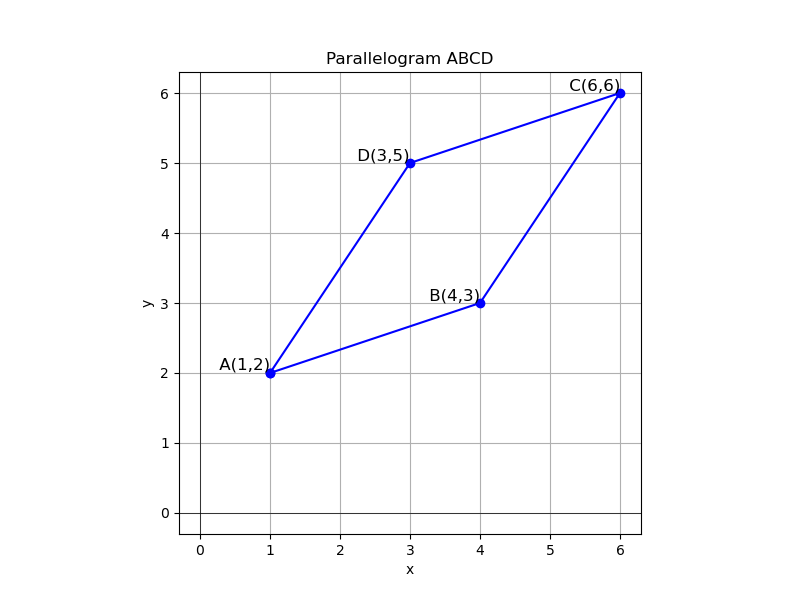
\includegraphics[width=0.7\linewidth]{Figure_1.png}
   \caption{Plot of parallelogram ABCD}
   \label{Parallelogram}
\end{figure}

\end{document}
